\chapter{Misurazioni e risultati}

\section{Tx\_Cx}
Si vuole simulare un ambiente in cui un nodo, facente le funzioni di server, vuole trasmettere un flusso di pacchetti verso un altro nodo che agirà come un client. 
Nei casi di test che successivamente saranno analizzati, i quattro dispositivi Rock che compongono il testbed verranno suddivisi in due gruppi separati, due in uno e i restanti due in un altro, ognuno con una funzione specifica.

I due gruppi saranno:

\begin{itemize}
    \item \textit{Gruppo Cx}: esso sarà composto da due dispositivi che simuleranno, con modalità che verranno discusse a breve, un ambiente in cui sono presenti uno svariato numero di veicoli che portano il canale di trasmissione a congestionarsi, in maniera completa o parziale.
    \item \textit{Gruppo Tx}: esso, invece, sarà composto da due dispositivi che comunicheranno mediante due flussi TCP in parallelo. Uno di essi agirà come client, che andrà a connettersi e a scaricare delle informazioni dall'altro che fungerà da server.
\end{itemize}

\begin{figure}[h!]
    \centering
    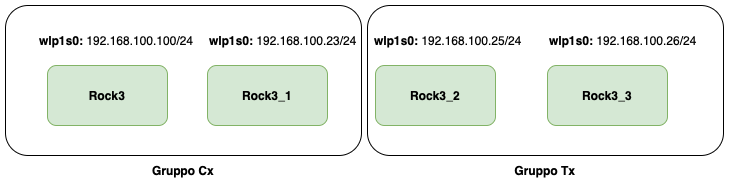
\includegraphics[width=1\textwidth]{diagramma_test.png}
    \caption{Diagramma dispositivi Rock}
    \label{fig:diagramma}
\end{figure}

Sono previsti tre principali casi di test:

\begin{itemize}
    \item \textit{T1\_C0}: assenza di QoS nei flussi dei dispositivi del \textit{Gruppo Tx} e assenza di congestione del canale, quindi il \textit{Gruppo Cx} sarà spento.
    \item \textit{T1\_C1}: assenza di QoS nei flussi dei dispositivi del \textit{Gruppo Tx} e totale congestione del canale, attuata mediante l'invio in broadcast di CAM da ognuno dei due dispositivi facenti parte del \textit{Gruppo Cx} ogni 5 ms.
    \item \textit{T1\_C2}: assenza di QoS nei flussi dei dispositivi del \textit{Gruppo Tx} e parziale congestione del canale, attuata mediante trasmissione UDP in \textit{flooding} in broadcast da parte di ognuno dei due dispositivi del \textit{Gruppo Cx}.
\end{itemize}

Questi stessi casi verranno, inoltre, ripetuti andando ad applicare delle politiche di QoS: un flusso verrà assegnato alla categoria con priorità maggiore, ovvero \textit{Access Category Voice} (AC\_VO), mentre l'altro alla categoria minore, ovvero \textit{Access Category Background} (AC\_BK).

Per fare ciò, viene utilizzato il comando iPerf, già precedentemente discusso, con i dovuti parametri. Nella fattispecie:

\begin{itemize}
    \item \textit{Rock Server}: \verb|iperf -s -i 1 -w 416K -y C -o output.csv|.
    \item \textit{Rock Client - flusso 1}: \\\verb|iperf -c 192.168.100.xxx -t 30 -b 10m -A VO| per il flusso a priorità maggiore.
    \item \textit{Rock Client - flusso 2}: \\\verb|iperf -c 192.168.100.xxx -t 30 -b 10m -A BK| per il flusso a priorità minore.
\end{itemize}

L'indirizzo IP usato nei due comandi è relativo a quello appartenente all'interfaccia \textit{wlp1s0} del dispositivo facente funzione di server.

Nei casi senza politiche di QoS sono stati utilizzati i medesimi comandi, senza ovviamente i parametri che delineano le varie priorità.

Per quanto concerne il raggiungimento di un eventuale congestione del canale, essa è stata raggiunta nei seguenti modi:

\begin{itemize}
    \item \textit{Caso senza congestione}: i dispositivi appartenenti al \textit{Gruppo Cx} non trasmettono alcunchè.
    \item \textit{Caso con congestione parziale}: i dispositivi appartenenti al \textit{Gruppo Cx}, come già detto poc'anzi, trasmettono ognuno un singolo pacchetto CAM ogni 5 ms; per tale scopo è stato lanciato sia su uno che sull'altro Rock lo script riportato in \autoref{udp_packets} con, come parametri, un \textit{message\_size} pari a 256 byte e lo \textit{sleep\_time} pari a 0.005; è stata scelto questo intervallo di tempo in quanto, tenendo conto che in caso di veicolo fermo esso invierebbe un CAM ogni 1 secondo, viene simulato un ambiente con 200 veicoli presenti.
    \item \textit{Caso con congestione totale}: i dispositivi appartenenti al \textit{Gruppo Cx} fanno flooding UDP mediante l'esecuzione del comando \verb|iperf -u -c 192.168.100.xxx| \verb| -t 300 -b 10m|; in questo caso si vuole simulare un ambiente con un numero veramente elevato di veicoli e molto maggiore del caso precedente.
\end{itemize}

In quest'ultimo caso, a causa delle limitazioni architetturali di iPerf, non è stato possibile inviare pacchetti UDP in broadcast. Poiché solo due dispositivi sono incaricati di effettuare flooding, la congestione viene raggiunta trasmettendo messaggi UDP da un dispositivo del \textit{Gruppo Cx} all'altro, specificando come parametro per iPerf l'indirizzo IP dell'interfaccia \textit{wlp1so} del Rock destinatario.

\subsection[T1 C1]{T1 C0}
Viene, qui, simulato un ambiente in cui non sono presenti veicoli di alcun tipo; di conseguenza non verranno trasmessi, in alcun modo, messaggi CAM. In questo contesto, inoltre, il dispositivo client, facente parte del \textit{gruppo Tx}, si connetterà per scaricare, mediante due flussi separati, delle informazioni dal dispositivo server.

In questo particolare caso, non verrà applicata alcuna politica di QoS e di conseguenza, ambedue i flussi avranno la medesima priorità.

Per fare ciò, viene utilizzato il comando iPerf, già precedentemente discusso, con i dovuti parametri. Nella fattispecie:

\begin{itemize}
    \item \textit{Rock Server}: \verb|iperf -s -i 1 -w 416K -y C -o output.csv|.
    \item \textit{Rock Client - flusso 1}: \verb|iperf -c 192.168.100.xxx -t 30 -b 10m| per quanto concerne il flusso 1.
    \item \textit{Rock Client - flusso 2}: \verb|iperf -c 192.168.100.xxx -t 30 -b 10m| per quanto concerne il flusso 2.
\end{itemize}

Alcune note particolari:

\begin{itemize}
    \item 
\end{itemize}

iperf senza qos con una connessione con due flussi tcp (t1 client e t2 server)
Caso senza congestione: c1 e c2 spenti

\begin{figure}[h!]
    \centering
    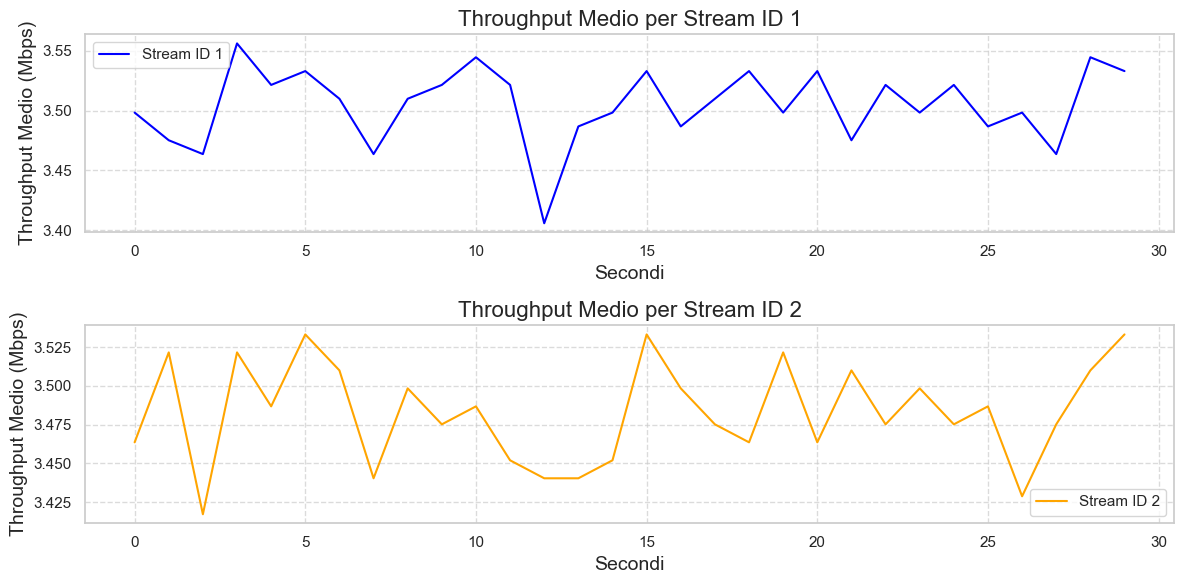
\includegraphics[width=1\textwidth]{t1_c0.png}
    \caption{Distributed Coordination Function}
    \label{fig:t1_c0}
\end{figure}

\subsection[T1 C1]{T1 C1}
iperf senza qos con una connessione con due flussi tcp (t1 client e t2 server)
Caso traffico stradale: c1 e c2 con cam ogni 5 ms in broadcast

\subsection[T1 C1]{T1 C2}
iperf senza qos con una connessione con due flussi tcp (t1 client e t2 server)
c1 client e c2 server con trasmissione udp in flooding

\subsection[T2 C1]{T1 C0}
come T1 ma usando VO e BK (t1 client e t2 server)
Caso senza congestione: c1 e c2 spenti

\subsection[T2 C1]{T1 C1}
come T1 ma usando VO e BK (t1 client e t2 server)
Caso traffico stradale: c1 e c2 con cam ogni 5 ms in broadcast

\subsection[T2 C1]{T1 C2}
come T1 ma usando VO e BK (t1 client e t2 server)
c1 client e c2 server con trasmissione udp in flooding
\section{Test 2}

\section{Lost packets}